\documentclass[11pt,a4paper]{article}
\usepackage[utf8]{inputenc}
\usepackage[T1]{fontenc}
\usepackage{lmodern}
\usepackage{babel}
\babelprovide[import,main]{spanish}
\addto\captionsspanish{\renewcommand{\tablename}{Tabla}}
\usepackage[margin=2.3cm]{geometry}
\usepackage{booktabs,tabularx,longtable,array}
\usepackage{enumitem}
\usepackage{amsmath,amssymb}
\usepackage{graphicx}
\usepackage{tikz}
\usetikzlibrary{arrows.meta,calc}
\usepackage{caption}
\usepackage[hidelinks]{hyperref}
\hypersetup{pdftitle={CPU multiciclo S-MIPS: informe de implementación y pruebas},pdfauthor={},pdfsubject={Arquitectura de Computadoras, curso 2026--2027}}
\setlist{itemsep=2pt,topsep=4pt}
\setlength{\emergencystretch}{3em}
\setlength{\LTcapwidth}{\linewidth}
\captionsetup{font=small,labelfont=normalfont,hypcap=false}
\newcommand{\sig}[1]{\texttt{#1}}
\newcommand{\estudiante}{\rule{6cm}{0.35pt}} % Sustituir por el nombre y los apellidos.
\newcommand{\curso}{Arquitectura de Computadoras --- Curso 2026--2027}
\title{CPU multiciclo S-MIPS en Logisim Evolution\\[4pt]\large Informe de implementación y pruebas}
\author{Estudiante: Héctor Sebastián Rodríguez Chacón\\[5pt]\normalsize\curso}
\date{}
\pdfmapfile{+lm.map}
\begin{document}
\maketitle

\section{Implementación y uso de VHDL}

La CPU se implementó con componentes de Logisim Evolution 5.0.0, sin VHDL,
para observar las señales y los registros durante la simulación. Integra
\sig{Instruction\_Decoder}, \sig{Control\_Unit}, \sig{Branch\_Control} y
\sig{Datapath}, con una sola ALU. Se conservaron \sig{Board}, \sig{Memory}
y los diez pines de la CPU. Los registros usan el mismo CLK y flanco ascendente;
la CPU no contiene RAM ni ROM \cite{guia,circuito}.

\section{Ruta de datos}

Las figuras~\ref{fig:operaciones} y~\ref{fig:memoria} representan dos partes
del mismo datapath. Los nombres repetidos identifican el mismo bus; las líneas
discontinuas indican controles. La memoria y el TTY pertenecen a la placa.

\begin{center}
\resizebox{\linewidth}{!}{% Panel 1. Incluir con \input{} dentro de un entorno figure.
% Requiere tikz y libraries arrows.meta,calc.
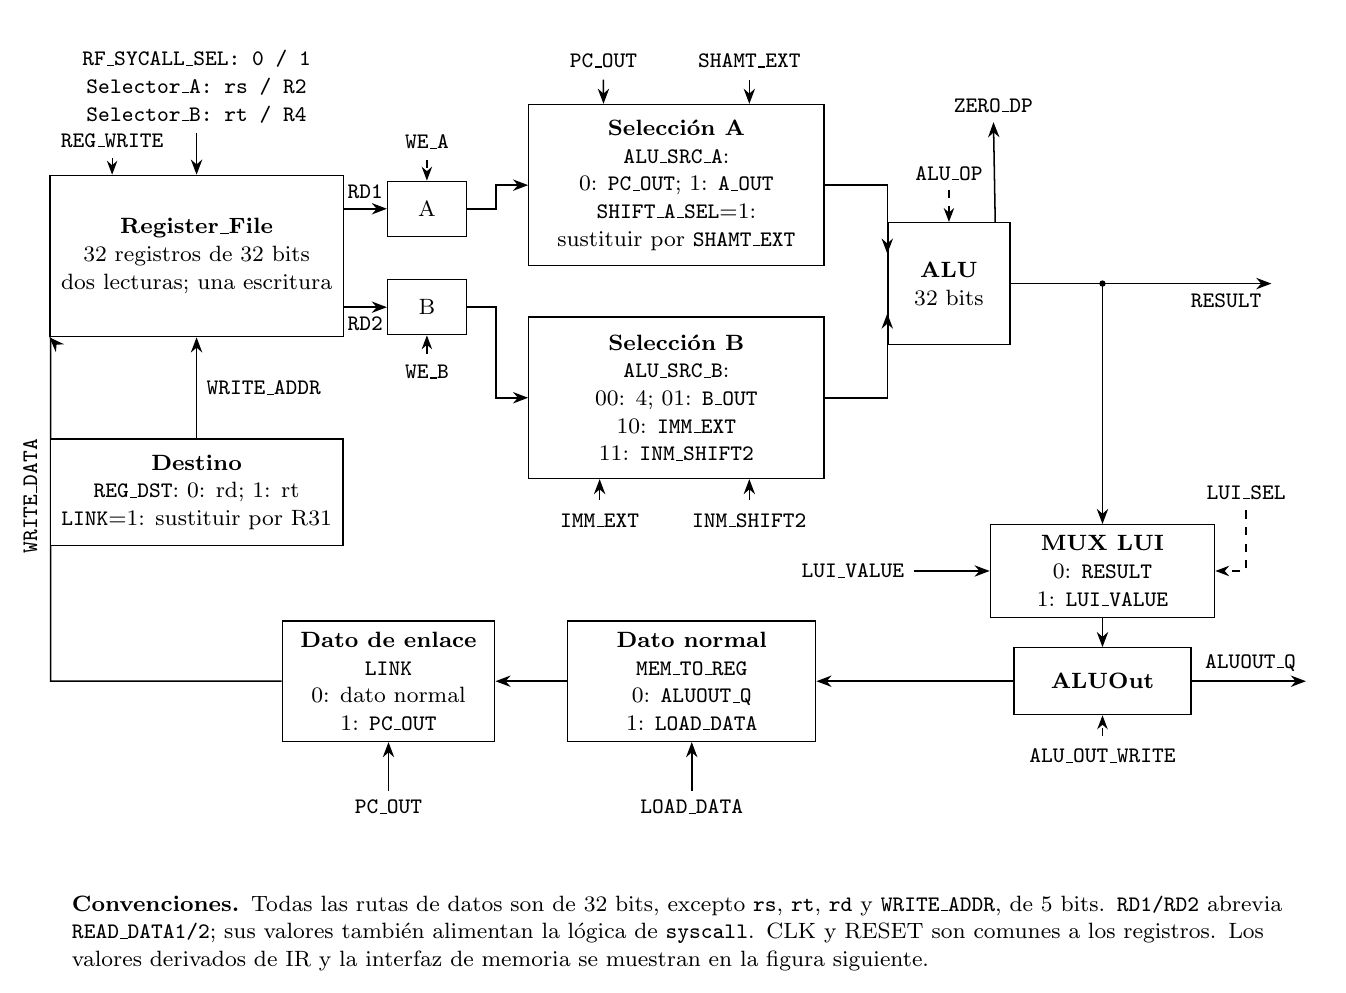
\begin{tikzpicture}[
  x=0.975cm,y=1cm,
  >=Stealth,
  every node/.style={font=\fontsize{8.5}{10}\selectfont},
  block/.style={draw,rectangle,align=center,inner sep=4pt,line width=.45pt,fill=white},
  reg/.style={block,minimum width=1.0cm,minimum height=.70cm},
  wire/.style={->,line width=.55pt},
  net/.style={font=\fontsize{8.5}{10}\selectfont\ttfamily,align=center},
  ctl/.style={font=\fontsize{8.5}{10}\selectfont\ttfamily,align=center},
  ctlwire/.style={->,dashed,line width=.45pt}
]
\path[use as bounding box] (-.45,-9.0) rectangle (16.35,2.9);

% Banco y registros de operandos.
\node[block,minimum width=3.50cm,minimum height=2.05cm] (rf) at (1.75,0)
  {\textbf{Register\_File}\\32 registros de 32 bits\\dos lecturas; una escritura};
\node[net] (selectors) at (1.75,2.15)
  {RF\_SYCALL\_SEL: 0 / 1\\Selector\_A: rs / R2\\Selector\_B: rt / R4};
\draw[wire] (selectors.south) -- (rf.north);

\node[reg] (ra) at (4.75,.60) {A};
\node[reg] (rb) at (4.75,-.65) {B};
\draw[wire] ($(rf.east)+(0,.60)$) -- node[above,net] {RD1} (ra.west);
\draw[wire] ($(rf.east)+(0,-.65)$) -- node[below,net] {RD2} (rb.west);
\node[ctl] at (4.75,1.45) {WE\_A};
\draw[ctlwire] (4.75,1.22) -- (ra.north);
\node[ctl] at (4.75,-1.47) {WE\_B};
\draw[ctlwire] (4.75,-1.24) -- (rb.south);

% Seleccion de operandos. Cada rectangulo describe exactamente los MUX indicados.
\node[block,minimum width=3.75cm,minimum height=2.05cm] (ma) at (8.0,.90)
 {\textbf{Selección A}\\
  \texttt{ALU\_SRC\_A}:\\
  0: \texttt{PC\_OUT}; 1: \texttt{A\_OUT}\\
  \texttt{SHIFT\_A\_SEL}=1:\\
  sustituir por \texttt{SHAMT\_EXT}};
\node[block,minimum width=3.75cm,minimum height=2.05cm] (mb) at (8.0,-1.80)
 {\textbf{Selección B}\\
  \texttt{ALU\_SRC\_B}:\\
  00: 4; 01: \texttt{B\_OUT}\\
  10: \texttt{IMM\_EXT}\\
  11: \texttt{INM\_SHIFT2}};
\draw[wire] (ra.east) -- (5.65,.60) |- (ma.west);
\draw[wire] (rb.east) -- (5.65,-.65) |- (mb.west);
\node[net,anchor=south] at (7.05,2.27) {PC\_OUT};
\draw[wire] (7.05,2.24) -- ($(ma.north)+(-.95,0)$);
\node[net,anchor=south] at (8.95,2.27) {SHAMT\_EXT};
\draw[wire] (8.95,2.24) -- ($(ma.north)+(.95,0)$);
\node[net,anchor=north] at (7.0,-3.15) {IMM\_EXT};
\draw[wire] (7.0,-3.10) -- ($(mb.south)+(-1.0,0)$);
\node[net,anchor=north] at (8.95,-3.15) {INM\_SHIFT2};
\draw[wire] (8.95,-3.10) -- ($(mb.south)+(.95,0)$);

% ALU, bypass LUI y registro temporal del resultado.
\node[block,minimum width=1.55cm,minimum height=1.55cm] (alu) at (11.55,-.35)
 {\textbf{ALU}\\32 bits};
\draw[wire] (ma.east) -| ($(alu.west)+(0,.38)$);
\draw[wire] (mb.east) -| ($(alu.west)+(0,-.38)$);
\node[ctl] (op) at (11.55,1.05) {ALU\_OP};
\draw[ctlwire] (op.south) -- (alu.north);
\draw[wire] (alu.east) -- (15.75,-.35) node[right,net,anchor=north east] {RESULT};
\coordinate (result) at (13.55,-.35);
\fill (result) circle (1.15pt);
\draw[wire] ($(alu.north east)+(-.20,0)$) -- (12.13,1.70)
  node[above,net] {ZERO\_DP};
\node[block,minimum width=2.85cm,minimum height=1.05cm] (mlui) at (13.55,-4.0)
 {\textbf{MUX LUI}\\0: \texttt{RESULT}\\1: \texttt{LUI\_VALUE}};
\draw[wire] (result) -- (mlui.north);
\node[ctl] at (15.42,-3.0) {LUI\_SEL};
\draw[ctlwire] (15.42,-3.23) |- (mlui.east);
\node[net] (lui) at (10.3,-4.0) {LUI\_VALUE};
\draw[wire] (lui.east) -- (mlui.west);
\node[block,minimum width=2.25cm,minimum height=.85cm] (ao) at (13.55,-5.40) {\textbf{ALUOut}};
\draw[wire] (mlui.south) -- (ao.north);
\node[ctl] at (13.55,-6.35) {ALU\_OUT\_WRITE};
\draw[ctlwire] (13.55,-6.10) -- (ao.south);
\draw[wire] (ao.east) -- (16.20,-5.40) node[above,net,anchor=south east] {ALUOUT\_Q};

% Ruta de writeback.
\node[block,minimum width=3.15cm,minimum height=1.45cm] (mwb) at (8.20,-5.40)
 {\textbf{Dato normal}\\\texttt{MEM\_TO\_REG}\\0: \texttt{ALUOUT\_Q}\\1: \texttt{LOAD\_DATA}};
\draw[wire] (ao.west) -- (mwb.east);
\node[net] (load) at (8.20,-7.0) {LOAD\_DATA};
\draw[wire] (load.north) -- (mwb.south);
\node[block,minimum width=2.70cm,minimum height=1.45cm] (mlink) at (4.25,-5.40)
 {\textbf{Dato de enlace}\\\texttt{LINK}\\0: dato normal\\1: \texttt{PC\_OUT}};
\draw[wire] (mwb.west) -- (mlink.east);
\node[net] (pcwb) at (4.25,-7.0) {PC\_OUT};
\draw[wire] (pcwb.north) -- (mlink.south);
\draw[wire] (mlink.west) -- (-.15,-5.40) -- (-.15,-1.05) -- (rf.south west);
\node[net,rotate=90,anchor=south] at (-.20,-3.05) {WRITE\_DATA};

% Destino y habilitacion del banco.
\node[block,minimum width=3.40cm,minimum height=1.35cm] (dst) at (1.75,-3.00)
 {\textbf{Destino}\\\texttt{REG\_DST}: 0: rd; 1: rt\\\texttt{LINK}=1: sustituir por R31};
\draw[wire] (dst.north) -- node[right,net] {WRITE\_ADDR} (rf.south);
\node[ctl] at (.65,1.47) {REG\_WRITE};
\draw[ctlwire] (.65,1.24) -- ($(rf.north)+(-1.10,0)$);

% Nombres de redes para cruzar con el otro panel.
\node[align=left,anchor=north west,text width=15.8cm] at (0,-8.0)
 {\textbf{Convenciones.} Todas las rutas de datos son de 32 bits, excepto
  \texttt{rs}, \texttt{rt}, \texttt{rd} y \texttt{WRITE\_ADDR}, de 5 bits.
  \texttt{RD1/RD2} abrevia \texttt{READ\_DATA1/2}; sus valores también alimentan
  la lógica de \texttt{syscall}. CLK y RESET son comunes a los registros.
  Los valores derivados de IR y la interfaz de memoria se muestran en la figura siguiente.};
\end{tikzpicture}
}
\captionof{figure}{Banco de registros, operandos, ALU y escritura del resultado.}
\label{fig:operaciones}
\end{center}

\clearpage
\subsection{PC, instrucción y acceso a memoria}

\begin{center}
\resizebox{\linewidth}{!}{% Panel 2. Incluir con \input{} dentro de un entorno figure.
% Requiere tikz y libraries arrows.meta,calc.
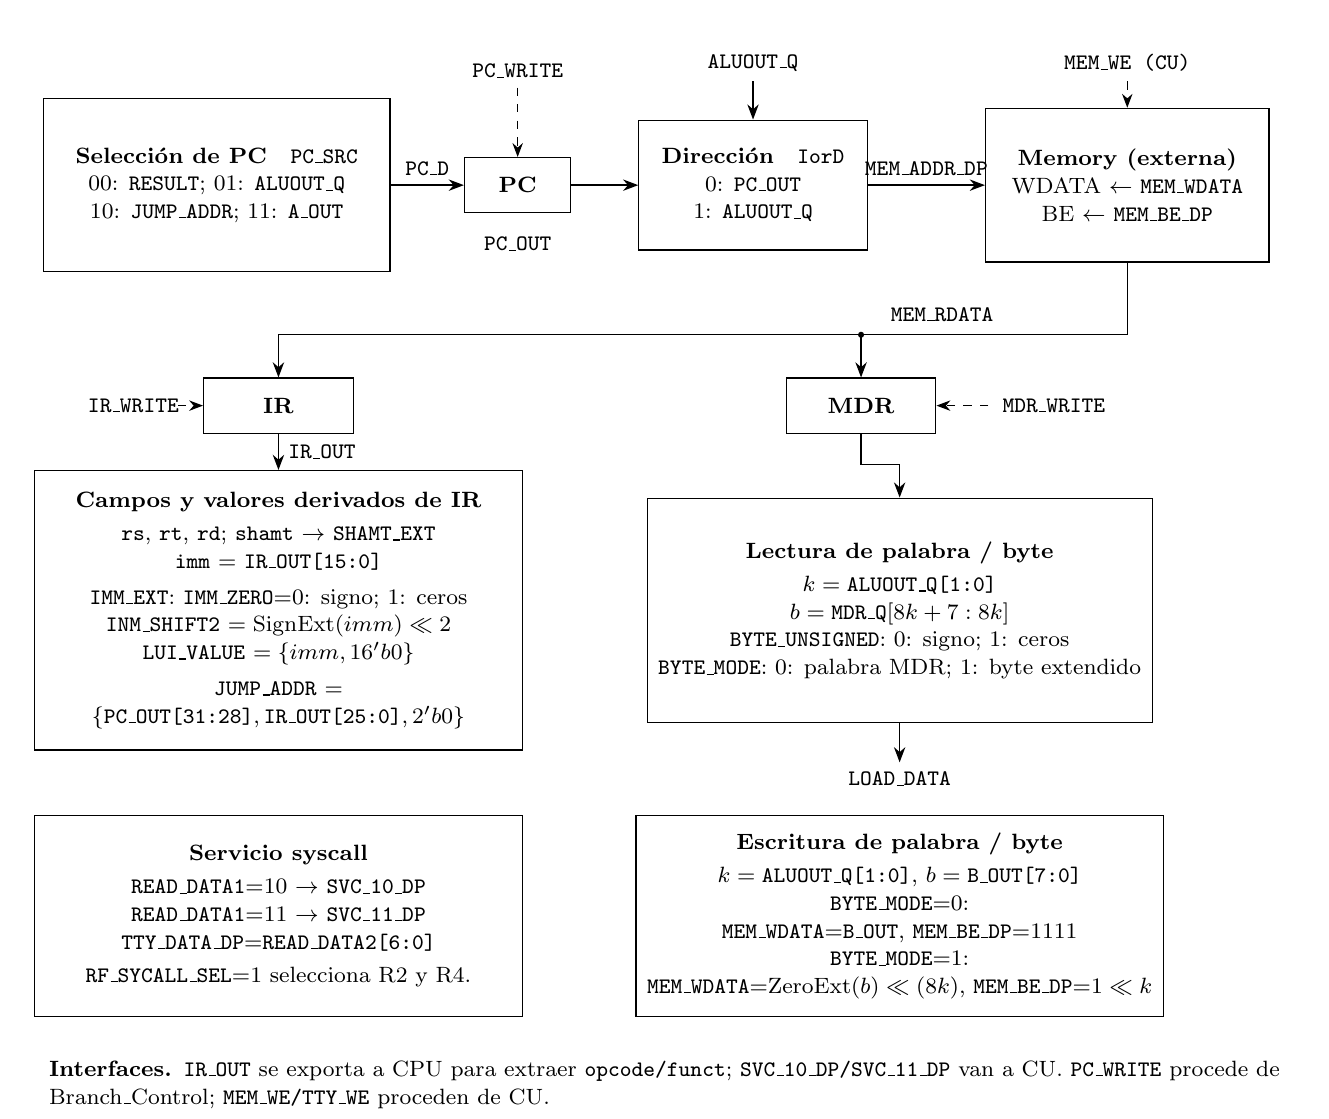
\begin{tikzpicture}[
  x=.98cm,y=1cm,>=Stealth,
  every node/.style={font=\fontsize{8.5}{10}\selectfont},
  block/.style={draw,rectangle,align=center,inner sep=4pt,line width=.45pt,fill=white},
  reg/.style={block,minimum width=1.35cm,minimum height=.70cm},
  wire/.style={->,line width=.55pt},
  net/.style={font=\fontsize{8.5}{10}\selectfont\ttfamily,align=center},
  ctl/.style={font=\fontsize{8.5}{10}\selectfont\ttfamily,align=center},
  ctlwire/.style={->,dashed,line width=.45pt}
]
\path[use as bounding box] (-.15,-11.35) rectangle (16.35,2.15);

% PC y seleccion de direccion.
\node[block,minimum width=4.40cm,minimum height=2.20cm] (mpc) at (2.30,.15)
 {\textbf{Selección de PC}\quad\texttt{PC\_SRC}\\
  00: \texttt{RESULT}; 01: \texttt{ALUOUT\_Q}\\
  10: \texttt{JUMP\_ADDR}; 11: \texttt{A\_OUT}};
\node[reg] (pc) at (6.20,.15) {\textbf{PC}};
\draw[wire] (mpc.east) -- node[above,net] {PC\_D} (pc.west);
\node[ctl] (pcw) at (6.20,1.60) {PC\_WRITE};
\draw[ctlwire] (pcw.south) -- (pc.north);
\node[block,minimum width=2.9cm,minimum height=1.65cm] (addr) at (9.25,.15)
 {\textbf{Dirección}\quad\texttt{IorD}\\
  0: \texttt{PC\_OUT}\\1: \texttt{ALUOUT\_Q}};
\draw[wire] (pc.east) -- (addr.west);
\node[net] at (6.20,-.60) {PC\_OUT};
\node[net] (aoadr) at (9.25,1.70) {ALUOUT\_Q};
\draw[wire] (aoadr.south) -- (addr.north);
\node[block,minimum width=3.60cm,minimum height=1.95cm] (mem) at (14.10,.15)
 {\textbf{Memory (externa)}\\
  WDATA $\leftarrow$ \texttt{MEM\_WDATA}\\
  BE $\leftarrow$ \texttt{MEM\_BE\_DP}};
\draw[wire] (addr.east) -- node[above,net] {MEM\_ADDR\_DP} (mem.west);
\node[ctl] (we) at (14.10,1.70) {MEM\_WE (CU)};
\draw[ctlwire] (we.south) -- (mem.north);

% Salida asíncrona de memoria: dos registros con habilitaciones independientes.
\coordinate (rbus) at (14.10,-1.75);
\draw (mem.south) -- (rbus) -- (3.10,-1.75);
\node[net,anchor=south] at (11.7,-1.70) {MEM\_RDATA};
\node[reg,minimum width=1.90cm] (ir) at (3.10,-2.65) {\textbf{IR}};
\node[reg,minimum width=1.90cm] (mdr) at (10.65,-2.65) {\textbf{MDR}};
\draw[wire] (3.10,-1.75) -- (ir.north);
\fill (10.65,-1.75) circle (1.1pt);
\draw[wire] (10.65,-1.75) -- (mdr.north);
\node[ctl] at (1.22,-2.65) {IR\_WRITE};
\draw[ctlwire] (1.8,-2.65) -- (ir.west);
\node[ctl] at (13.15,-2.65) {MDR\_WRITE};
\draw[ctlwire] (12.30,-2.65) -- (mdr.east);

% Extracción de campos y formación de operandos sin sumadores adicionales.
\node[block,minimum width=6.20cm,minimum height=3.55cm] (imm) at (3.10,-5.25)
 {\textbf{Campos y valores derivados de IR}\\[2pt]
  \texttt{rs}, \texttt{rt}, \texttt{rd}; \texttt{shamt} $\to$ \texttt{SHAMT\_EXT}\\
  \texttt{imm} $=$ \texttt{IR\_OUT[15:0]}\\[3pt]
  \texttt{IMM\_EXT}: \texttt{IMM\_ZERO}=0: signo; 1: ceros\\
  \texttt{INM\_SHIFT2} $= \operatorname{SignExt}(imm) \ll 2$\\
  \texttt{LUI\_VALUE} $= \{imm,16'b0\}$\\[3pt]
  \texttt{JUMP\_ADDR} $=$\\
  $\{\texttt{PC\_OUT[31:28]},\texttt{IR\_OUT[25:0]},2'b0\}$};
\draw[wire] (ir.south) -- node[right,net] {IR\_OUT} (imm.north);

% LOAD: seleccionar carril antes de extender.
\node[block,minimum width=6.20cm,minimum height=2.85cm] (ld) at (11.15,-5.25)
 {\textbf{Lectura de palabra / byte}\\[2pt]
  $k=\texttt{ALUOUT\_Q[1:0]}$\\
  $b=\texttt{MDR\_Q}[8k+7:8k]$\\
  \texttt{BYTE\_UNSIGNED}: 0: signo; 1: ceros\\
  \texttt{BYTE\_MODE}: 0: palabra MDR; 1: byte extendido};
\draw[wire] (mdr.south) -- (10.65,-3.40) -| (ld.north);
\draw[wire] (ld.south) -- (11.15,-7.18) node[below,net] {LOAD\_DATA};

% SYS: toma puertos de lectura vivos, no los registros A/B.
\node[block,minimum width=6.20cm,minimum height=2.55cm] (svc) at (3.10,-9.13)
 {\textbf{Servicio syscall}\\[2pt]
  \texttt{READ\_DATA1}=10 $\to$ \texttt{SVC\_10\_DP}\\
  \texttt{READ\_DATA1}=11 $\to$ \texttt{SVC\_11\_DP}\\
  \texttt{TTY\_DATA\_DP}=\texttt{READ\_DATA2[6:0]}\\[2pt]
  \texttt{RF\_SYCALL\_SEL}=1 selecciona R2 y R4.};

% STORE: byte bajo de B alineado por el offset.
\node[block,minimum width=6.20cm,minimum height=2.55cm] (st) at (11.15,-9.13)
 {\textbf{Escritura de palabra / byte}\\[2pt]
  $k=\texttt{ALUOUT\_Q[1:0]}$, $b=\texttt{B\_OUT[7:0]}$\\
  \texttt{BYTE\_MODE}=0:\\
  \texttt{MEM\_WDATA}=\texttt{B\_OUT}, \texttt{MEM\_BE\_DP}=1111\\
  \texttt{BYTE\_MODE}=1:\\
  \texttt{MEM\_WDATA}=$\operatorname{ZeroExt}(b)\ll(8k)$, \texttt{MEM\_BE\_DP}=$1\ll k$};

\node[align=left,anchor=north west,text width=15.9cm] at (0,-10.85)
 {\textbf{Interfaces.} \texttt{IR\_OUT} se exporta a CPU para extraer \texttt{opcode/funct};
  \texttt{SVC\_10\_DP/SVC\_11\_DP} van a CU.
  \texttt{PC\_WRITE} procede de Branch\_Control;
  \texttt{MEM\_WE/TTY\_WE} proceden de CU.};
\end{tikzpicture}
}
\captionof{figure}{Selección del PC, memoria compartida, campos del IR y tratamiento de bytes.}
\label{fig:memoria}
\end{center}

\sig{IR} conserva la instrucción mientras se ejecuta. Los registros A y B
conservan sus operandos; \sig{ALUOut} guarda resultados o direcciones, y
\sig{MDR} guarda la palabra leída. Los campos \sig{rs}, \sig{rt} y \sig{rd}
tienen 5 bits; \sig{shamt}, 5; el inmediato, 16; \sig{op} y \sig{funct}, 6.
El inmediato se extiende a 32 bits con signo o ceros. Para \sig{lui} se forma
$\{IR[15{:}0],16'b0\}$ y se selecciona antes de \sig{ALUOut}.

La memoria contiene 4096 palabras de 32 bits y usa orden \emph{little-endian}.
\sig{MEM\_ADDR[13:2]} selecciona la palabra y los dos bits inferiores
seleccionan el byte. Para \sig{lb}/\sig{lbu}, el byte de MDR se extiende con
signo/ceros; para \sig{sb}, se coloca B[7:0] en el carril seleccionado y se
activa únicamente su bit de \sig{MEM\_BE}. \sig{sw} activa los cuatro bits.

\sig{RESET} establece PC=0, R28=\sig{0x1800}, R29=\sig{0x3FFC} y los demás
registros arquitectónicos a cero. La inicialización del banco se asegura
manteniendo RESET durante un flanco ascendente. R0 siempre se lee como cero
y la memoria de la placa no se borra mediante RESET.

\clearpage
\section{Máquina de estados}

El estado se codifica con 5 bits. La tabla~\ref{tab:fsm} muestra los 18 estados
utilizados; los códigos se expresan en hexadecimal. En FETCH se captura IR y
se guarda PC+4 en ALUOut. El PC se actualiza en DECODE, si la instrucción es
legal. Por ello, los estados posteriores ya disponen del PC incrementado.

\begin{center}
\small\setlength{\tabcolsep}{4pt}
\begin{tabularx}{\linewidth}{@{}l l l X@{}}
\toprule
Código & Estado & Siguiente & Operación principal \\
\midrule
\sig{00} & \sig{FETCH} & 01 & IR $\leftarrow$ memoria; ALUOut $\leftarrow$ PC+4 \\
\sig{01} & \sig{DECODE} & Según clase & Si es legal: A/B $\leftarrow$ RF; PC $\leftarrow$ ALUOut \\
\sig{02} & \sig{EXEC\_R} & 06 & ALUOut $\leftarrow$ operación R \\
\sig{03} & \sig{EXEC\_I} & 06 & ALUOut $\leftarrow$ operación con inmediato \\
\sig{04} & \sig{EXEC\_SHIFT} & 06 & ALUOut $\leftarrow$ desplazamiento de B \\
\sig{05} & \sig{EXEC\_LUI} & 06 & ALUOut $\leftarrow$ $\{imm16,16\text{ ceros}\}$ \\
\sig{06} & \sig{WB\_ALU} & 00 & RF $\leftarrow$ ALUOut \\
\sig{07} & \sig{MEM\_ADDR} & 08 / 0A & ALUOut $\leftarrow$ A + SignExt(imm) \\
\sig{08} & \sig{MEM\_READ} & 09 & MDR $\leftarrow$ palabra de memoria \\
\sig{09} & \sig{MEM\_WB} & 00 & RF[rt] $\leftarrow$ LOAD\_DATA \\
\sig{0A} & \sig{MEM\_WRITE} & 00 & Memoria $\leftarrow$ B, palabra o byte \\
\sig{0B} & \sig{BR\_TARGET} & 0C & ALUOut $\leftarrow$ PC + (SignExt(imm) $\ll$ 2) \\
\sig{0C} & \sig{BR\_COMPARE} & 00 & Comparar A$-$B; actualizar PC si procede \\
\sig{0D} & \sig{JUMP} & 00 & PC $\leftarrow$ JUMP\_ADDR; enlace en jal \\
\sig{0E} & \sig{JR} & 00 & PC $\leftarrow$ A\_OUT \\
\sig{0F} & \sig{SYSCALL\_CHECK} & 1F / 10 / 00 & Examinar el servicio de R2 \\
\sig{10} & \sig{SYSCALL\_PRINT} & 00 & Escribir R4[6:0] en el TTY \\
\sig{1F} & \sig{HALT} & 1F & Conservar el estado hasta RESET \\
\bottomrule
\end{tabularx}
\captionof{table}{Estados y transiciones de la unidad de control.}\label{tab:fsm}
\end{center}

En DECODE, las instrucciones R aritméticas pasan a \sig{02}; las inmediatas,
a \sig{03}; los desplazamientos, a \sig{04}; \sig{lui}, a \sig{05}; las
cargas y stores, a \sig{07}; los branches, a \sig{0B}; \sig{j}/\sig{jal},
a \sig{0D}; \sig{jr}, a \sig{0E}; y \sig{syscall}, a \sig{0F}. Una
instrucción ilegal pasa a \sig{1F} sin escribir A, B ni PC. Como
\sig{IS\_JUMP} también incluye \sig{jr}, \sig{IS\_JR} tiene prioridad
para seleccionar su recorrido.

Desde \sig{07}, \sig{IS\_LOAD} selecciona \sig{08} y \sig{IS\_STORE}
selecciona \sig{0A}. En \sig{0F}, R2=10 lleva a HALT; R2=11, a
\sig{SYSCALL\_PRINT}; cualquier otro servicio vuelve a FETCH sin efecto.
HALT se mantiene hasta RESET. RESET fuerza el estado \sig{00}; los estados
no utilizados, \sig{11}--\sig{1E}, regresan a FETCH.

\sig{PC\_WRITE} es una
salida de \sig{Branch\_Control}, obtenida mediante
\begin{align*}
\sig{BRANCH\_TAKEN}&=(\sig{BEQ\_EN}\land\sig{ZERO})
 \lor(\sig{BNE\_EN}\land\neg\sig{ZERO}),\\
\sig{PC\_WRITE}&=\sig{PC\_ADVANCE}\lor\sig{JUMP\_EN}\lor\sig{BRANCH\_TAKEN}.
\end{align*}

\clearpage
\section{Señales de control por estado}

Las tablas siguientes documentan las 28 salidas de \sig{Control\_Unit}.
Se supone \sig{RESET=0}; su efecto se precisa al final del apartado.
Las condiciones que aparecen en las celdas son
\[
i=\sig{IS\_ILLEGAL},\qquad \ell=\neg i,\qquad
j=\sig{IS\_JAL},\qquad n=\sig{IS\_BNE}.
\]

\subsection{Escrituras, parada y cambios del PC}
\begin{center}
\footnotesize
\setlength{\tabcolsep}{5.4pt}
\begin{tabular}{@{}lccccccccc@{}}
\toprule
Estado & IRW & AW & BW & OW & MW & RW & MemW & TTYW & H \\
\midrule
\texttt{00} & \texttt{1} & \texttt{0} & \texttt{0} & \texttt{1} & \texttt{0} & \texttt{0} & \texttt{0} & \texttt{0} & \texttt{0} \\
\texttt{01} & \texttt{0} & $\ell$ & $\ell$ & \texttt{0} & \texttt{0} & \texttt{0} & \texttt{0} & \texttt{0} & \texttt{0} \\
\texttt{02} & \texttt{0} & \texttt{0} & \texttt{0} & \texttt{1} & \texttt{0} & \texttt{0} & \texttt{0} & \texttt{0} & \texttt{0} \\
\texttt{03} & \texttt{0} & \texttt{0} & \texttt{0} & \texttt{1} & \texttt{0} & \texttt{0} & \texttt{0} & \texttt{0} & \texttt{0} \\
\texttt{04} & \texttt{0} & \texttt{0} & \texttt{0} & \texttt{1} & \texttt{0} & \texttt{0} & \texttt{0} & \texttt{0} & \texttt{0} \\
\texttt{05} & \texttt{0} & \texttt{0} & \texttt{0} & \texttt{1} & \texttt{0} & \texttt{0} & \texttt{0} & \texttt{0} & \texttt{0} \\
\texttt{06} & \texttt{0} & \texttt{0} & \texttt{0} & \texttt{0} & \texttt{0} & \texttt{1} & \texttt{0} & \texttt{0} & \texttt{0} \\
\texttt{07} & \texttt{0} & \texttt{0} & \texttt{0} & \texttt{1} & \texttt{0} & \texttt{0} & \texttt{0} & \texttt{0} & \texttt{0} \\
\texttt{08} & \texttt{0} & \texttt{0} & \texttt{0} & \texttt{0} & \texttt{1} & \texttt{0} & \texttt{0} & \texttt{0} & \texttt{0} \\
\texttt{09} & \texttt{0} & \texttt{0} & \texttt{0} & \texttt{0} & \texttt{0} & \texttt{1} & \texttt{0} & \texttt{0} & \texttt{0} \\
\texttt{0A} & \texttt{0} & \texttt{0} & \texttt{0} & \texttt{0} & \texttt{0} & \texttt{0} & \texttt{1} & \texttt{0} & \texttt{0} \\
\texttt{0B} & \texttt{0} & \texttt{0} & \texttt{0} & \texttt{1} & \texttt{0} & \texttt{0} & \texttt{0} & \texttt{0} & \texttt{0} \\
\texttt{0C} & \texttt{0} & \texttt{0} & \texttt{0} & \texttt{0} & \texttt{0} & \texttt{0} & \texttt{0} & \texttt{0} & \texttt{0} \\
\texttt{0D} & \texttt{0} & \texttt{0} & \texttt{0} & \texttt{0} & \texttt{0} & $j$ & \texttt{0} & \texttt{0} & \texttt{0} \\
\texttt{0E} & \texttt{0} & \texttt{0} & \texttt{0} & \texttt{0} & \texttt{0} & \texttt{0} & \texttt{0} & \texttt{0} & \texttt{0} \\
\texttt{0F} & \texttt{0} & \texttt{0} & \texttt{0} & \texttt{0} & \texttt{0} & \texttt{0} & \texttt{0} & \texttt{0} & \texttt{0} \\
\texttt{10} & \texttt{0} & \texttt{0} & \texttt{0} & \texttt{0} & \texttt{0} & \texttt{0} & \texttt{0} & \texttt{1} & \texttt{0} \\
\texttt{1F} & \texttt{0} & \texttt{0} & \texttt{0} & \texttt{0} & \texttt{0} & \texttt{0} & \texttt{0} & \texttt{0} & \texttt{1} \\
\bottomrule
\end{tabular}
\captionof{table}{Habilitaciones de escritura y salida de parada, con RESET=0.}\label{tab:escrituras}
\end{center}

En la tabla~\ref{tab:escrituras}, IRW, AW, BW, OW, MW y RW representan
\sig{IR\_WRITE}, \sig{A\_WRITE}, \sig{B\_WRITE}, \sig{ALUOUT\_WRITE},
\sig{MDR\_WRITE} y \sig{REG\_WRITE}. MemW, TTYW y H corresponden a
\sig{MEM\_WE}, \sig{TTY\_WE} y \sig{HALT}.

\begin{center}
\footnotesize
\setlength{\tabcolsep}{5.4pt}
\begin{tabular}{@{}lccccccc@{}}
\toprule
Estado & PA & IH & BEQ & BNE & JE & LINK & SC \\
\midrule
\texttt{00} & \texttt{0} & \texttt{0} & \texttt{0} & \texttt{0} & \texttt{0} & \texttt{0} & \texttt{0} \\
\texttt{01} & $\ell$ & $i$ & \texttt{0} & \texttt{0} & \texttt{0} & \texttt{0} & \texttt{0} \\
\texttt{02} & \texttt{0} & \texttt{0} & \texttt{0} & \texttt{0} & \texttt{0} & \texttt{0} & \texttt{0} \\
\texttt{03} & \texttt{0} & \texttt{0} & \texttt{0} & \texttt{0} & \texttt{0} & \texttt{0} & \texttt{0} \\
\texttt{04} & \texttt{0} & \texttt{0} & \texttt{0} & \texttt{0} & \texttt{0} & \texttt{0} & \texttt{0} \\
\texttt{05} & \texttt{0} & \texttt{0} & \texttt{0} & \texttt{0} & \texttt{0} & \texttt{0} & \texttt{0} \\
\texttt{06} & \texttt{0} & \texttt{0} & \texttt{0} & \texttt{0} & \texttt{0} & \texttt{0} & \texttt{0} \\
\texttt{07} & \texttt{0} & \texttt{0} & \texttt{0} & \texttt{0} & \texttt{0} & \texttt{0} & \texttt{0} \\
\texttt{08} & \texttt{0} & \texttt{0} & \texttt{0} & \texttt{0} & \texttt{0} & \texttt{0} & \texttt{0} \\
\texttt{09} & \texttt{0} & \texttt{0} & \texttt{0} & \texttt{0} & \texttt{0} & \texttt{0} & \texttt{0} \\
\texttt{0A} & \texttt{0} & \texttt{0} & \texttt{0} & \texttt{0} & \texttt{0} & \texttt{0} & \texttt{0} \\
\texttt{0B} & \texttt{0} & \texttt{0} & \texttt{0} & \texttt{0} & \texttt{0} & \texttt{0} & \texttt{0} \\
\texttt{0C} & \texttt{0} & \texttt{0} & $\neg n$ & $n$ & \texttt{0} & \texttt{0} & \texttt{0} \\
\texttt{0D} & \texttt{0} & \texttt{0} & \texttt{0} & \texttt{0} & \texttt{1} & $j$ & \texttt{0} \\
\texttt{0E} & \texttt{0} & \texttt{0} & \texttt{0} & \texttt{0} & \texttt{1} & \texttt{0} & \texttt{0} \\
\texttt{0F} & \texttt{0} & \texttt{0} & \texttt{0} & \texttt{0} & \texttt{0} & \texttt{0} & \texttt{1} \\
\texttt{10} & \texttt{0} & \texttt{0} & \texttt{0} & \texttt{0} & \texttt{0} & \texttt{0} & \texttt{1} \\
\texttt{1F} & \texttt{0} & \texttt{0} & \texttt{0} & \texttt{0} & \texttt{0} & \texttt{0} & \texttt{0} \\
\bottomrule
\end{tabular}
\captionof{table}{Control de cambios del PC, enlace y acceso a registros de syscall.}\label{tab:pc}
\end{center}

{\raggedright
PA=\sig{PC\_ADVANCE}, IH=\sig{ILLEGAL\_HALT}, BEQ=\sig{BEQ\_EN},
BNE=\sig{BNE\_EN}, JE=\sig{JUMP\_EN} y SC=\sig{REF\_SYCALL\_SEL}.
Se conservan los nombres literales del circuito.\par}



\clearpage
\subsection{Selectores y controles dependientes de la instrucción}

Sea $a=\sig{ALU\_OP\_DEC}$, de 3 bits. En la tabla~\ref{tab:selectores},
PCS, AS~A, AS~B, M2R, SH y LUI representan \sig{PC\_SRC},
\sig{ALU\_SRC\_A}, \sig{ALU\_SRC\_B}, \sig{MEM\_TO\_REG},
\sig{SHIFT\_A\_SEL} y \sig{LUI\_SEL}, respectivamente.

\begin{center}
\small
\setlength{\tabcolsep}{5.4pt}
\begin{tabular}{@{}lcccccccc@{}}
\toprule
Estado & PCS & AS A & AS B & ALU OP & IorD & M2R & SH & LUI \\
\midrule
\texttt{00} & \texttt{00} & \texttt{0} & \texttt{00} & \texttt{000} & \texttt{0} & \texttt{0} & \texttt{0} & \texttt{0} \\
\texttt{01} & \texttt{01} & \texttt{0} & \texttt{00} & \texttt{000} & \texttt{0} & \texttt{0} & \texttt{0} & \texttt{0} \\
\texttt{02} & \texttt{00} & \texttt{1} & \texttt{01} & $a$ & \texttt{0} & \texttt{0} & \texttt{0} & \texttt{0} \\
\texttt{03} & \texttt{00} & \texttt{1} & \texttt{10} & $a$ & \texttt{0} & \texttt{0} & \texttt{0} & \texttt{0} \\
\texttt{04} & \texttt{00} & \texttt{0} & \texttt{01} & $a$ & \texttt{0} & \texttt{0} & \texttt{1} & \texttt{0} \\
\texttt{05} & \texttt{00} & \texttt{0} & \texttt{00} & \texttt{000} & \texttt{0} & \texttt{0} & \texttt{0} & \texttt{1} \\
\texttt{06} & \texttt{00} & \texttt{0} & \texttt{00} & \texttt{000} & \texttt{0} & \texttt{0} & \texttt{0} & \texttt{0} \\
\texttt{07} & \texttt{00} & \texttt{1} & \texttt{10} & \texttt{000} & \texttt{0} & \texttt{0} & \texttt{0} & \texttt{0} \\
\texttt{08} & \texttt{00} & \texttt{0} & \texttt{00} & \texttt{000} & \texttt{1} & \texttt{0} & \texttt{0} & \texttt{0} \\
\texttt{09} & \texttt{00} & \texttt{0} & \texttt{00} & \texttt{000} & \texttt{0} & \texttt{1} & \texttt{0} & \texttt{0} \\
\texttt{0A} & \texttt{00} & \texttt{0} & \texttt{00} & \texttt{000} & \texttt{1} & \texttt{0} & \texttt{0} & \texttt{0} \\
\texttt{0B} & \texttt{00} & \texttt{0} & \texttt{11} & \texttt{000} & \texttt{0} & \texttt{0} & \texttt{0} & \texttt{0} \\
\texttt{0C} & \texttt{01} & \texttt{1} & \texttt{01} & \texttt{001} & \texttt{0} & \texttt{0} & \texttt{0} & \texttt{0} \\
\texttt{0D} & \texttt{10} & \texttt{0} & \texttt{00} & \texttt{000} & \texttt{0} & \texttt{0} & \texttt{0} & \texttt{0} \\
\texttt{0E} & \texttt{11} & \texttt{0} & \texttt{00} & \texttt{000} & \texttt{0} & \texttt{0} & \texttt{0} & \texttt{0} \\
\texttt{0F} & \texttt{00} & \texttt{0} & \texttt{00} & \texttt{000} & \texttt{0} & \texttt{0} & \texttt{0} & \texttt{0} \\
\texttt{10} & \texttt{00} & \texttt{0} & \texttt{00} & \texttt{000} & \texttt{0} & \texttt{0} & \texttt{0} & \texttt{0} \\
\texttt{1F} & \texttt{00} & \texttt{0} & \texttt{00} & \texttt{000} & \texttt{0} & \texttt{0} & \texttt{0} & \texttt{0} \\
\bottomrule
\end{tabular}
\captionof{table}{Valores físicos de los selectores. Los ceros se muestran incluso cuando la ruta no se consume.}\label{tab:selectores}
\end{center}

Las cuatro salidas restantes tienen el mismo significado en todos los estados:
\begin{align*}
\sig{REG\_DST}&=\sig{IS\_ALU\_I}\lor\sig{IS\_LUI}\lor\sig{IS\_LOAD},\\
\sig{IMM\_ZERO}&=\sig{EXT\_MODE\_DEC}[0],\\
\sig{BYTE\_MODE}&=\sig{IS\_BYTE},\qquad
\sig{BYTE\_UNSIGNED}=\sig{IS\_LBU}.
\end{align*}

\begin{center}
\small\setlength{\tabcolsep}{5pt}
\begin{tabularx}{\linewidth}{@{}l X@{}}
\toprule
Selector & Correspondencia entre código y entrada \\
\midrule
\sig{ALU\_SRC\_A} & 0: PC\_OUT; 1: A\_OUT. Después, SHIFT\_A\_SEL=1 sustituye el dato por SHAMT\_EXT. \\
\sig{ALU\_SRC\_B} & 00: 4; 01: B\_OUT; 10: IMM\_EXT; 11: INM\_SHIFT2. \\
\sig{PC\_SRC} & 00: ALU.RESULT; 01: ALUOUT\_Q; 10: JUMP\_ADDR; 11: A\_OUT. \\
\sig{IorD} & 0: PC\_OUT; 1: ALUOUT\_Q. \\
\sig{REG\_DST} & 0: rd; 1: rt. LINK=1 sustituye después el destino por R31. \\
\sig{MEM\_TO\_REG} & 0: ALUOUT\_Q; 1: LOAD\_DATA. LINK=1 sustituye después el dato por PC\_OUT. \\
\sig{LUI\_SEL} & 0: ALU.RESULT; 1: LUI\_VALUE. \\
\bottomrule
\end{tabularx}
\captionof{table}{Selección de las rutas principales.}
\end{center}

En SHIFT, \sig{ALU\_SRC\_A=0} y \sig{SHIFT\_A\_SEL=1}. En \sig{jal},
\sig{REG\_DST=MEM\_TO\_REG=0}; R31 y PC\_OUT se seleccionan mediante
los MUX adicionales de LINK. Estos datos no son valores de los selectores
de un bit.

\paragraph{Reset.} Las máscaras explícitas son
$\sig{MEM\_WE}=[q=\sig{0A}]\land\neg\sig{RESET}$,
$\sig{TTY\_WE}=[q=\sig{10}]\land\neg\sig{RESET}$ y
$\sig{HALT}=[q=\sig{1F}]\land\neg\sig{RESET}$.
Las salidas asociadas al estado adoptan los valores de FETCH cuando RESET
lleva el estado a 00; por ejemplo, IR\_WRITE y ALUOUT\_WRITE valen 1.
Los cuatro controles dependientes de la instrucción siguen las ecuaciones anteriores.

\clearpage
\section{Codificación de la ALU y del decodificador}

\subsection{Operaciones de la ALU}

La ALU recibe dos operandos de 32 bits y un código de 3 bits. Las sumas y
restas producen resultados de 32 bits; \sig{slt} compara con signo. Los
desplazamientos actúan sobre B y utilizan A[4:0] como cantidad de posiciones.
\sig{ZERO} vale 1 si los 32 bits del resultado son cero.

\begin{center}\small
\begin{tabular}{@{}cll@{}}
\toprule Código & Operación & Resultado \\\midrule
\sig{000} & ADD & $A+B$ \\
\sig{001} & SUB & $A-B$ \\
\sig{010} & AND & $A\land B$ \\
\sig{011} & OR & $A\lor B$ \\
\sig{100} & SLT & $A<B$ con signo: palabra 1 o 0 \\
\sig{101} & SLL & $B\ll A[4{:}0]$ \\
\sig{110} & SRL & Desplazamiento lógico de B a la derecha \\
\bottomrule
\end{tabular}
\captionof{table}{Codificación de ALU\_OP. El código 111 no se utiliza.}
\end{center}

\subsection{Salidas de Instruction\_Decoder}

El decodificador es combinacional: recibe \sig{OP[5:0]} y
\sig{FUNCT[5:0]}. Produce dos buses y quince indicadores de un bit. La tabla
siguiente define todas sus salidas; las abreviaturas se utilizan en la
tabla~\ref{tab:isa}.

\begin{center}\small\setlength{\tabcolsep}{4pt}
\begin{tabularx}{\linewidth}{@{}l c X@{}}
\toprule Salida & Bits / abrev. & Significado \\\midrule
\sig{ALU\_OP\_DEC} & 3 & Código de operación para EXEC\_R, EXEC\_I y EXEC\_SHIFT. \\
\sig{EXT\_MODE\_DEC} & 2 & 00: signo; 01: ceros; 10: LUI. \\
\sig{IS\_ALU\_R} & 1 / R & add, addu, sub, and, or, slt. \\
\sig{IS\_ALU\_I} & 1 / I & addi, addiu, slti, andi, ori. \\
\sig{IS\_SHIFT} & 1 / SH & sll, srl. \\
\sig{IS\_LOAD} & 1 / LD & lw, lb, lbu. \\
\sig{IS\_STORE} & 1 / ST & sw, sb. \\
\sig{IS\_BYTE} & 1 / BY & lb, lbu, sb. \\
\sig{IS\_BRANCH} & 1 / BR & beq, bne. \\
\sig{IS\_JUMP} & 1 / JP & j, jal y jr. \\
\sig{IS\_LUI} & 1 / LU & lui. \\
\sig{IS\_LBU} & 1 / BU & lbu. \\
\sig{IS\_BNE} & 1 / NE & bne. \\
\sig{IS\_JAL} & 1 / JL & jal. \\
\sig{IS\_JR} & 1 / JR & jr. \\
\sig{IS\_SYCALL} & 1 / SC & syscall; nombre literal del pin. \\
\sig{IS\_ILLEGAL} & 1 & Ninguna de las codificaciones admitidas. \\
\bottomrule
\end{tabularx}
\captionof{table}{Las diecisiete salidas del decodificador.}
\end{center}

\sig{addiu} usa extensión de signo, igual que \sig{addi}. En \sig{lui},
\sig{EXT\_MODE\_DEC=10} y \sig{IMM\_ZERO=0}; el resultado se obtiene
por la ruta \sig{LUI\_VALUE}, seleccionada mediante \sig{LUI\_SEL}.
Para \sig{beq}/\sig{bne}, \sig{ALU\_OP\_DEC=000}; es la CU la que fuerza
\sig{ALU\_OP=001} durante BR\_COMPARE.

\clearpage
\subsection{Correspondencia entre instrucción y salidas}

\sig{OP} y \sig{FUNCT} se indican en hexadecimal; los dos buses de salida,
en binario. Los indicadores enumerados valen 1 y los demás valen 0.
\sig{IS\_ILLEGAL=0} en todas estas filas. Cuando OP no es 00, FUNCT no
interviene en la identificación de la instrucción.

\begin{center}\small\setlength{\tabcolsep}{5pt}
\begin{tabularx}{\linewidth}{@{}l c c c c X@{}}
\toprule
Instrucción & OP & FUNCT & ALU\_OP\_DEC & EXT\_MODE\_DEC & Indicadores \\
\midrule
\sig{add} & \sig{00} & \texttt{20} & \sig{000} & \sig{00} & R \\
\sig{addu} & \sig{00} & \texttt{21} & \sig{000} & \sig{00} & R \\
\sig{sub} & \sig{00} & \texttt{22} & \sig{001} & \sig{00} & R \\
\sig{and} & \sig{00} & \texttt{24} & \sig{010} & \sig{00} & R \\
\sig{or} & \sig{00} & \texttt{25} & \sig{011} & \sig{00} & R \\
\sig{slt} & \sig{00} & \texttt{2A} & \sig{100} & \sig{00} & R \\
\sig{sll} & \sig{00} & \texttt{00} & \sig{101} & \sig{00} & SH \\
\sig{srl} & \sig{00} & \texttt{02} & \sig{110} & \sig{00} & SH \\
\sig{jr} & \sig{00} & \texttt{08} & \sig{000} & \sig{00} & JP, JR \\
\sig{syscall} & \sig{00} & \texttt{0C} & \sig{000} & \sig{00} & SC \\
\sig{addi} & \sig{08} & --- & \sig{000} & \sig{00} & I \\
\sig{addiu} & \sig{09} & --- & \sig{000} & \sig{00} & I \\
\sig{slti} & \sig{0A} & --- & \sig{100} & \sig{00} & I \\
\sig{andi} & \sig{0C} & --- & \sig{010} & \sig{01} & I \\
\sig{ori} & \sig{0D} & --- & \sig{011} & \sig{01} & I \\
\sig{lui} & \sig{0F} & --- & \sig{000} & \sig{10} & LU \\
\sig{lw} & \sig{23} & --- & \sig{000} & \sig{00} & LD \\
\sig{lb} & \sig{20} & --- & \sig{000} & \sig{00} & LD, BY \\
\sig{lbu} & \sig{24} & --- & \sig{000} & \sig{00} & LD, BY, BU \\
\sig{sw} & \sig{2B} & --- & \sig{000} & \sig{00} & ST \\
\sig{sb} & \sig{28} & --- & \sig{000} & \sig{00} & ST, BY \\
\sig{beq} & \sig{04} & --- & \sig{000} & \sig{00} & BR \\
\sig{bne} & \sig{05} & --- & \sig{000} & \sig{00} & BR, NE \\
\sig{j} & \sig{02} & --- & \sig{000} & \sig{00} & JP \\
\sig{jal} & \sig{03} & --- & \sig{000} & \sig{00} & JP, JL \\
\bottomrule
\end{tabularx}
\captionof{table}{Codificaciones reconocidas y salidas del decodificador.}\label{tab:isa}
\end{center}

La palabra \sig{0x00000000} se interpreta como
\sig{sll \$zero,\$zero,0}; es legal y actúa como \sig{nop}. Una combinación
no admitida activa \sig{IS\_ILLEGAL}. No se exige que los campos no usados
de una instrucción válida sean cero, de acuerdo con la guía.

\section{Ciclos por clase de instrucción}

Se cuenta desde FETCH hasta completar la instrucción, sin incluir el FETCH
de la siguiente ni los ciclos de reset. En una parada se cuenta el flanco
que hace entrar a HALT.

\begin{center}\small\setlength{\tabcolsep}{5pt}
\begin{tabularx}{\linewidth}{@{}l X c@{}}
\toprule Clase & Recorrido después de FETCH y DECODE & Ciclos \\\midrule
ALU R/I, shift, lui & EXEC correspondiente; WB\_ALU & 4 \\
lw, lb, lbu & MEM\_ADDR; MEM\_READ; MEM\_WB & 5 \\
sw, sb & MEM\_ADDR; MEM\_WRITE & 4 \\
beq, bne & BR\_TARGET; BR\_COMPARE & 4 \\
j, jal, jr & JUMP o JR & 3 \\
syscall 11 & SYSCALL\_CHECK; SYSCALL\_PRINT & 4 \\
syscall 10 / otro & SYSCALL\_CHECK; entrar a HALT / FETCH & 3 \\
Ilegal & Entrar a HALT al finalizar DECODE & 2 \\\bottomrule
\end{tabularx}
\captionof{table}{Número de ciclos por instrucción.}
\end{center}

\clearpage
\section{Cobertura de los programas propios}

Se conservaron los cinco programas originales de \sig{tests/}. La
tabla~\ref{tab:cobertura} relaciona sus instrucciones con las dieciséis filas
de casos exigidas por la tabla 3 de la guía. Los programas de \sig{programs/}
aportan comprobaciones adicionales, pero se distinguen de las pruebas propias.

\begin{table}[htbp]
\centering
\small
\caption{Correspondencia entre los casos de la tabla 3 de la guía y las pruebas propias.}
\label{tab:cobertura}
\begin{tabularx}{\linewidth}{@{}p{2.2cm}X p{4.35cm}@{}}
\toprule
Instrucciones & Caso ejecutado & Programa en \texttt{tests/} \\
\midrule
\texttt{add, sub} & Operandos positivos y al menos un operando negativo. & \texttt{arithmetic\_basic.asm} \\
\texttt{and, or} & Operandos con unos en los 16 bits altos. & \texttt{logic\_shifts.asm} \\
\texttt{slt, slti} & Resultados 1 y 0; negativo que distingue comparación con y sin signo. & \texttt{logic\_shifts.asm} \\
\texttt{sll, srl} & shamt=0 y shamt distinto de 0; SRL sobre un valor negativo. & \texttt{logic\_shifts.asm} \\
\texttt{addi} & Inmediato negativo. & \texttt{arithmetic\_basic.asm} \\
\texttt{addiu, addu} & Expansiones de li con constante de 16 bits y move. & \texttt{arithmetic\_basic.asm} \\
\texttt{andi, ori} & Inmediato cuyo bit 15 vale 1. & \texttt{logic\_shifts.asm} \\
\texttt{lui} & Inmediato cuyo bit 15 vale 1. & \texttt{logic\_shifts.asm} \\
\texttt{lw, sw} & Desplazamientos positivo y negativo. & \texttt{memory\_edges.asm} \\
\texttt{lb, lbu} & Bytes con bit 7 igual a 1 en dos posiciones distintas. & \texttt{memory\_edges.asm} \\
\texttt{sb} & Cuatro posiciones de una palabra; LW comprueba los otros bytes. & \texttt{memory\_edges.asm} \\
\texttt{beq, bne} & Cada uno tomado y no tomado; un salto hacia atrás. & \texttt{branch\_edges.asm} \\
\texttt{j} & Salto incondicional. & \texttt{branch\_edges.asm} \\
\texttt{jal, jr} & Procedimiento no hoja, RA guardado en pila y retorno. & \texttt{nested\_calls.asm} \\
\texttt{syscall} & Servicios 11 y 10. & Todos los tests \\
\texttt{\$zero} & Intento de escritura y comprobación posterior de cero. & \texttt{arithmetic\_basic.asm} \\
\bottomrule
\end{tabularx}
\end{table}


\subsection{Comprobación del ensamblado y de las salidas}

Las cinco imágenes contienen 221 instrucciones máquina: 33 de
\sig{arithmetic\_basic}, 41 de \sig{branch\_edges}, 59 de
\sig{logic\_shifts}, 60 de \sig{memory\_edges} y 28 de
\sig{nested\_calls}. Entre ellas aparecen las 25 operaciones requeridas.
En \sig{arithmetic\_basic}, las cinco \sig{li} se traducen a cinco
\sig{addiu} y el \sig{move} se traduce a \sig{addu}. Así se comprueban las
instrucciones emitidas por MARS, además del código fuente.

\begin{center}\small
\begin{tabular}{@{}ll@{}}
\toprule Prueba & Salida calculada, antes del salto de línea \\\midrule
\sig{arithmetic\_basic.asm} & \sig{95442210} \\
\sig{branch\_edges.asm} & \sig{010147} \\
\sig{logic\_shifts.asm} & \sig{18001361101010} \\
\sig{memory\_edges.asm} & \sig{1111111111} \\
\sig{nested\_calls.asm} & \sig{493} \\\bottomrule
\end{tabular}
\captionof{table}{Salidas de las pruebas propias.}
\end{center}

Todas caben en el TTY de 12 líneas de 48 caracteres. Los indicadores de
\sig{memory\_edges} dependen de comparaciones de los datos leídos y los
esperados. Las limitaciones de observación de estas pruebas se indican en
el apartado siguiente.

\clearpage
\section{Resultados y limitaciones}

Los resultados de la tabla~\ref{tab:resultados} corresponden al registro
\sig{salida-tests.txt} del repositorio \cite{resultados}. Se ejecutó la
batería completa con \sig{tools/run\_tests.py}, que ensambla los programas,
obtiene su salida en MARS y la compara con el TTY de la placa. El criterio
de éxito exige alcanzar HALT antes del límite de 60\,000 ciclos y que los
textos coincidan después de normalizar los espacios finales.

\begin{table}[htbp]
\centering
\small
\caption{Resultados registrados de la batería completa.}
\label{tab:resultados}
\begin{tabular}{@{}lrr@{}}
\toprule
Programa & Ciclos & Resultado \\
\midrule
\texttt{programs/arithmetic.asm} & 6795 & Correcto \\
\texttt{programs/array\_sum.asm} & 957 & Correcto \\
\texttt{programs/branches.asm} & 934 & Correcto \\
\texttt{programs/gcd.asm} & 3005 & Correcto \\
\texttt{programs/hello.asm} & 308 & Correcto \\
\texttt{programs/memory.asm} & 5174 & Correcto \\
\texttt{programs/multiply.asm} & 2064 & Correcto \\
\midrule
\texttt{tests/arithmetic\_basic.asm} & 131 & Correcto \\
\texttt{tests/branch\_edges.asm} & 174 & Correcto \\
\texttt{tests/logic\_shifts.asm} & 235 & Correcto \\
\texttt{tests/memory\_edges.asm} & 445 & Correcto \\
\texttt{tests/nested\_calls.asm} & 109 & Correcto \\
\midrule
Total & & 12/12 \\
\bottomrule
\end{tabular}
\end{table}


El resultado fue \textbf{12/12 correctos}: siete programas proporcionados
y cinco propios. Se comprobó además la ejecución manual de \sig{hello.hex}
en Board. No se identificaron fallos funcionales del micro en los programas
ejecutados; los ciclos corresponden al programa completo, incluidas sus
rutinas de impresión.

\subsection{Alcance de la validación}

La batería no es exhaustiva. Algunas pruebas propias muestran solo parte
del resultado de 32 bits; por ello, ciertos errores hipotéticos de extensión
del inmediato, OR o LUI podrían no modificar la salida. Asimismo, escribir
y leer con el mismo desplazamiento negativo puede ocultar un error
simétrico en el cálculo de la dirección. Son limitaciones de las
comprobaciones, no fallos observados en el circuito actual.

El ejecutor verifica el texto final y la llegada a HALT; no compara todos
los registros y posiciones de memoria ni verifica por sí solo que HALT se
mantenga estable en ciclos posteriores. La guía deja fuera de las pruebas
los accesos no alineados, los saltos no alineados, el desbordamiento de
\sig{add}/\sig{addi}/\sig{sub} que haría detenerse a MARS y los accesos
fuera de los 16 KiB. El procesador no implementa excepciones para esas
situaciones.

\begin{thebibliography}{3}
\small
\bibitem{guia} \emph{Proyecto: CPU multiciclo S-MIPS en Logisim Evolution.
Orientación y especificación}. Arquitectura de Computadoras,
curso 2026--2027. Requisitos R1--R23.
\bibitem{circuito} Repositorio \emph{Proyecto-S-MIPS-2026-2027},
versión \sig{c2ce80d}. Archivo \sig{circuit/smips.circ}.\\
\url{https://github.com/hectorsebastian2025/Proyecto-S-MIPS-2026-2027}
\bibitem{resultados} Mismo repositorio: \sig{salida-tests.txt},
\sig{tests/*.asm}, \sig{programs/*.asm} y \sig{tools/run\_tests.py}.
\end{thebibliography}
\end{document}
